\documentclass[paper=a4, fontsize=11pt]{scrartcl} % A4 paper and 11pt font size

\usepackage[T1]{fontenc} % Use 8-bit encoding that has 256 glyphs
\usepackage[english]{babel} % English language/hyphenation
\usepackage{amsmath,amsfonts,amsthm} % Math packages

\usepackage{graphicx}
\usepackage{placeins}

\usepackage{sectsty} % Allows customizing section commands
\allsectionsfont{\centering \normalfont\scshape} % Make all sections centered, the default font and small caps

\usepackage{fancyhdr} % Custom headers and footers
\pagestyle{fancyplain} % Makes all pages in the document conform to the custom headers and footers
\fancyhead{} % No page header - if you want one, create it in the same way as the footers below
\fancyfoot[L]{} % Empty left footer
\fancyfoot[C]{} % Empty center footer
\fancyfoot[R]{\thepage} % Page numbering for right footer
\renewcommand{\headrulewidth}{0pt} % Remove header underlines
\renewcommand{\footrulewidth}{0pt} % Remove footer underlines
\setlength{\headheight}{13.6pt} % Customize the height of the header

\numberwithin{equation}{section} % Number equations within sections (i.e. 1.1, 1.2, 2.1, 2.2 instead of 1, 2, 3, 4)
\numberwithin{figure}{section} % Number figures within sections (i.e. 1.1, 1.2, 2.1, 2.2 instead of 1, 2, 3, 4)
\numberwithin{table}{section} % Number tables within sections (i.e. 1.1, 1.2, 2.1, 2.2 instead of 1, 2, 3, 4)

\setlength\parindent{0pt} % Removes all indentation from paragraphs - comment this line for an assignment with lots of text

\newcommand{\horrule}[1]{\rule{\linewidth}{#1}} % Create horizontal rule command with 1 argument of height

\usepackage[noend]{algorithmic}
\usepackage[boxed]{algorithm}
\usepackage{url}
\usepackage{subfigure}
\usepackage{placeins}
\newcommand{\matr}[1]{\mathbf{#1}}

\title{	
\normalfont \normalsize 
\textsc{Boston University} \\ [25pt] % Your university, school and/or department name(s)
\horrule{0.5pt} \\[0.4cm] % Thin top horizontal rule
\huge EC500: Final Project \\
\horrule{2pt} \\[0.5cm] % Thick bottom horizontal rule
}

\author{Ariya Shajii, Huy Le, Winston Chen}

\date{\normalsize\today}

\begin{document}

\maketitle


\section{Introduction}

In this project, we solve in two dimensions the heat equation

\begin{equation}
	\rho c_p {\partial T \over \partial t} - \nabla \cdot (k \nabla T) = \dot{q},
	\label{eq:main}
\end{equation}

where

\begin{itemize}
	\item $k$ is a constant taken to be $1$,
	\item $\rho$ is the density of the medium (assumed to be constant),
	\item $c_p$ is the specific heat of the medium (assumed to be constant),
	\item $\dot{q}$ is the heat flux as a function of spacial coordinates $(x,y)$, and
	\item $T$ is the temperature of the material as a function of spatial coordinates $(x,y)$ and of time $t$.
\end{itemize}

In discrete form, the equation can be written as follows:

\begin{equation}
	\rho c_p (T_{x,y,t+1} - T_{x,y,t}) -
	k (T_{x+1,y,t} + T_{x-1,y,t} + T_{x,y+1,t} + T_{x,y-1,t} - 4T_{x,y,t}) = \dot{q}.
\end{equation}

The time step and spatial step have both been taken to be $1$ in the finite difference approximations. \linebreak

We now solve this problem using three different approaches:

\begin{itemize}
	\item Red-black iteration, parallelized with OpenMP and MPI
	\item Conjugate gradient method
	\item Using a triangular lattice instead of a conventional square lattice
\end{itemize}


\section{Parallelized Red-Black}


\section{Conjugate Gradient Method}

In order to use conjugate gradient (CG), we must write our problem in the form $\matr{A}\vec{x} = \vec{b}$ for vectors $\vec{x}$, $\vec{b}$ and matrix $\matr{A}$. In this case, $\vec{x}$ will be our temperature $T$, $\vec{b}$ will be our heat flux $\dot{q}$ and $\matr{A}$ will encode the left-hand side of Equation \ref{eq:main}. Note that we take ${\partial T \over \partial t} = 0$ since we are only interested in the steady-state solution when using CG. We are therefore left with:

\begin{equation}
	\matr{A}T_{x,y} = 4T_{x,y} - (T_{x+1,y} + T_{x-1,y} + T_{x,y+1} + T_{x,y-1}) = \vec{b} = \dot{q}.
	\label{eq:matrix}
\end{equation}

Note that we make the time variable $t$ implicit, since we no longer need it directly. The CG algorithm can now be applied as follows \footnote{Adapted from \url{https://en.wikipedia.org/wiki/Conjugate_gradient_method#The_resulting_algorithm}}:

\begin{algorithm}[H]
\caption{Conjugate gradient algorithm}
\begin{algorithmic}
	\REQUIRE{$\matr{A}$, $\vec{b}$, $\epsilon$}
	\ENSURE{$T$}
	\STATE $T \gets \vec{0}$
	\STATE $\vec{r} \gets \vec{b} - \matr{A}T$  \COMMENT{residual}
	\STATE $\vec{p} \gets \vec{r}$
	\LOOP
		\STATE $\alpha \gets \frac{|\vec{r}|}{\vec{p} \cdot \matr{A}\vec{p}}$
		\STATE $T \gets T + \alpha \vec{p}$
		\STATE $\vec{r}_{\mathrm{new}} \gets \vec{r} - \alpha\matr{A}\vec{p}$
		\IF {$|\vec{r}_{\mathrm{new}}| < \epsilon$}
			\RETURN $T$
		\ENDIF
		\STATE $\beta \gets \frac{|\vec{r}_{\mathrm{new}}|}{|\vec{r}|}$
		\STATE $p \gets \vec{r}_{\mathrm{new}} + \beta\vec{p}$
		\STATE $\vec{r} \gets \vec{r}_{\mathrm{new}}$
	\ENDLOOP
\end{algorithmic}
\label{alg:cg}
\end{algorithm}

We take our initial guess $T_0$ to be zero everywhere. All that Algorithm \ref{alg:cg} requires us to have is a way to perform dot products and a way of applying $\matr{A}$ to a vector. The former is fairly trivial and the latter is given by Equation \ref{eq:matrix}. With these fundamental operations at hand, it is straightforward to implement Algorithm \ref{alg:cg} in code. \linebreak

Quick note on boundary conditions: We incorporate our boundary conditions in $\vec{b}$ and apply $\matr{A}$ only to the interior points of $T$ -- that is, points that have exactly four neighbors.

\subsection{Results}

\begin{figure}
\centering
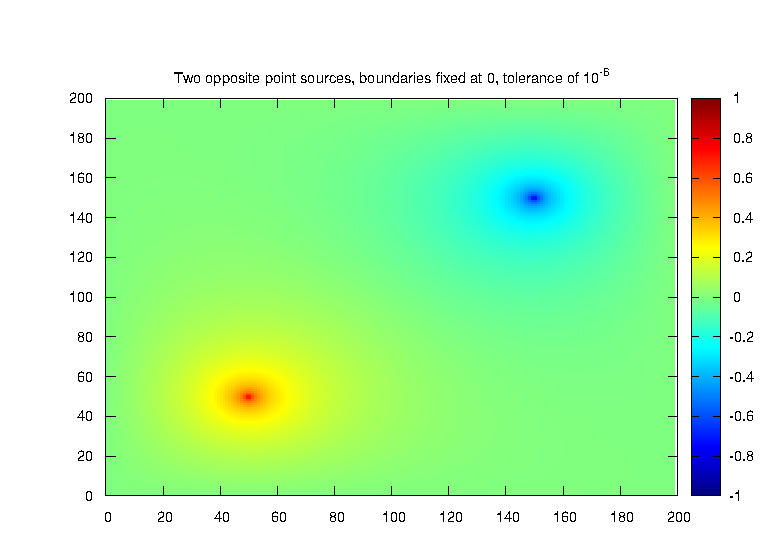
\includegraphics[width=400px]{heatmap1.eps}
\caption{Final heat map for system with two point sources as shown, with boundaries fixed at zero. The point sources are equal in magnitude but opposite in sign.}
\label{fig:cgheatmap}
\end{figure}

\begin{figure}
\centering
\subfigure[$k = 1$]{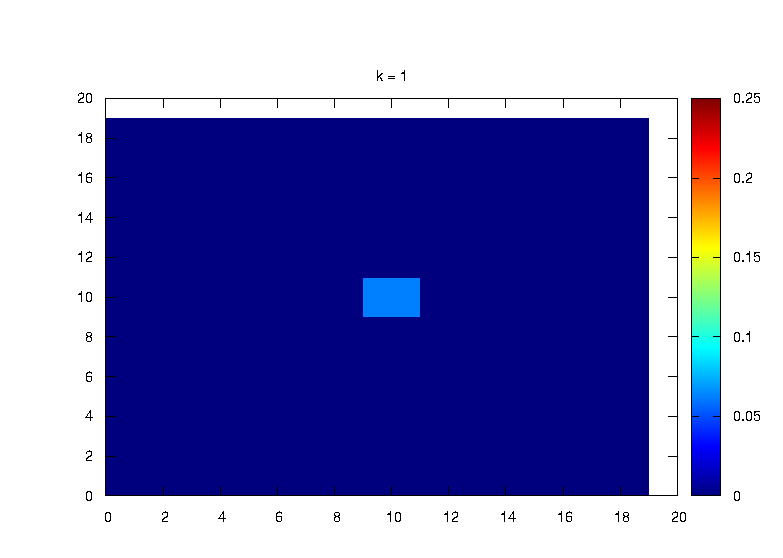
\includegraphics[width=60mm]{step_1.eps}}
\subfigure[$k = 2$]{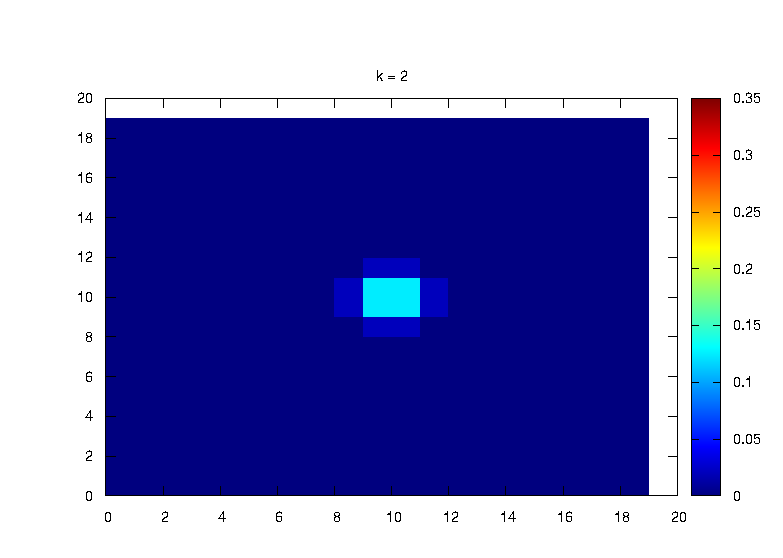
\includegraphics[width=60mm]{step_2.eps}}
\hfill
\subfigure[$k = 3$]{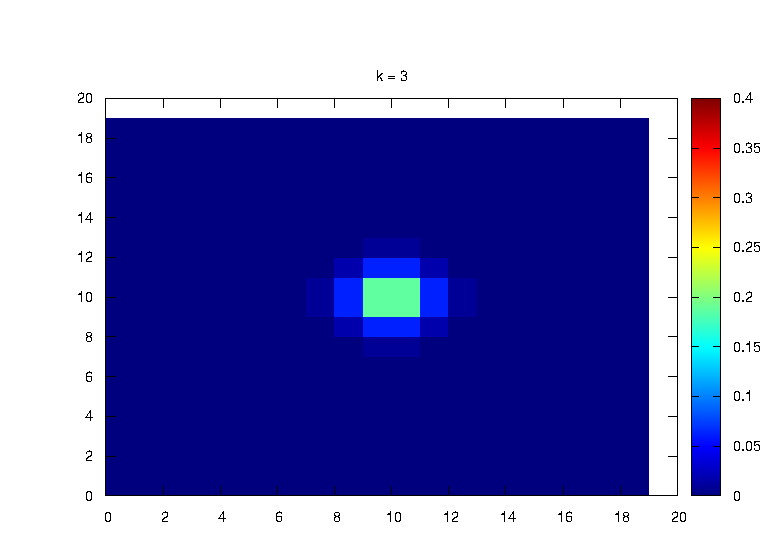
\includegraphics[width=60mm]{step_3.eps}}
\subfigure[$k = 4$]{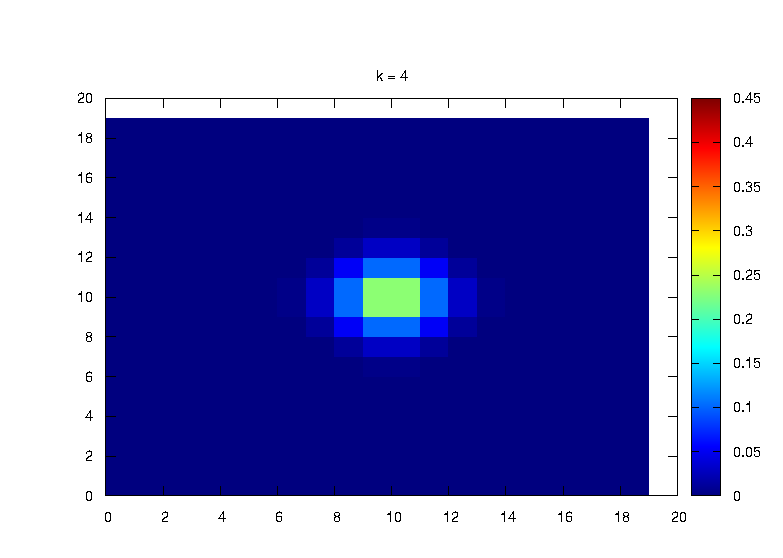
\includegraphics[width=60mm]{step_4.eps}}
\caption{First four steps of conjugate gradient algorithm for system with a single point source in the center.}
\label{fig:cgsteps}
\end{figure}

Figure \ref{fig:cgheatmap} shows the result of applying the CG algorithm to a system with two opposite point sources on a 200-by-200 grid. The boundaries were fixed at zero and a residual tolerance of $10^{-6}$ was used. It is also instructive to view the result after each of the first few iterations of the main loop in Algorithm \ref{alg:cg}. Consider a simpler system with a single point source in the center on a 20-by-20 grid. The result after the first four iterations is shown in Figure \ref{fig:cgsteps}. We can see from this figure how information propagates neighbor-by-neighbor from the source to the surrounding points. This makes sense since, by Equation \ref{eq:matrix}, each non-zero point can only influence its closest neighbors on each iteration.


\section{Triangular Lattice}


\section{Miscellaneous}
\subsection{Code}
The code for our project can be found at \url{https://github.com/winstonchen/ec500}.

\subsection{Contributions}
\begin{itemize}
	\item Ariya Shajii -- Conjugate gradient
	\item Huy Le -- Parallelized red-black iteration
	\item Winston Chen -- Triangular lattice
\end{itemize}

\end{document}
















